%\chapter*{knx}

\section{Introduction to KNX}

\gls{knx} implements a specialized form of automated process control, dedicated to the needs of home
and building automation. KNX emerged from 3 leading standards, namely the \gls{eib}, the \gls{ehs} and BatiBUS. It is an open, platform independent standard,
developed by the KNX association implementing the EN50090 standard for home and building electronic systems.

To provide platform independence, the standard uses a layered structure, based on the \gls{iso} / \gls{osi}.

\subsection{Datapoints}

Datapoints represent the process- and control variables of the system, and can be of
inputtype, outputtype, diagnostic data, parameters or others. To achieve interoperability,
Datapoints are grouped into functional blocks, implementing standardized datapoint types.

\section{KNX Layers}

The \gls{osi} standardizes the communication between different, independent systems
by grouping the needed functions into 7 sublayers to provide interchangeability and abstraction. Every layer provides services to its next-higher layer, and
uses the services provided by its next-lower layer. Every service is defined by standardized interfaces - that way any layer can be modified internally without
compromising the function of the system, as long as the defined interfaces are implemented. This fragmentation of one service follows the paradigm of 
\textit{impera et divide}\footnote{latin:  \textit{dive and rule}} and facilitates the building of complex systems by dividing one complex problem into subsequent,
less-complex problems.

KNX implements this model, omitting 
layers 5 and 6, as shown in figure \ref{fig:knxlayers}. Data from applications are directly passed to the transport layer in a transparent way, and vice versa.

\begin{figure}
    \centering
    \includegraphics[width=0.8\textwidth]{figures/"knx vs iso layers".png}
    \caption{OSI Layer Model, compared to the KNX Model}
    \label{fig:knxlayers}
\end{figure}

\subsection{Physical Layer}

This is the lowest layer as defined by \gls{osi} and determines the basic transmission parameters like symbol rate, signal form but also mechanical 
characteristics like which connectors are used.

To provide flexibility in \gls{knx}, 4 different physical media are defined. \gls{TP}-1 which was inherited from \gls{eib}, and is the successor of \gls{TP}-0,
as defined by BatiBUS, is the basis medium, consisting of a twisted pair cabeling. Data and power can be transmitted with one pair, so low-power
devices can be fed over the bus. Data transfer is done asynchronously, with bidirectional, half-duplex
 communication and a datarate of 9600 bit/sec. \gls{TP}-1 uses collision avoidance, and allows all topologies beside rings. 
 
Because this work is base on the \gls{TP}1 - part of KNX only, this medium will be explained in more detail in the next chapter.
\\

PL110, which was also inherited from \gls{eib}, uses the power line for communications. The carrier uses spread frequency shift keying, and can be used 
for bidirectional, half duplex  communication with an even lower data rate of 1200 bit/sec
\\

\gls{knx} \gls{rf} is used for short range wireless communication at 868,3 MHz. 
\\

\gls{knx} \gls{IP} allows the integration of \gls{knx} into the the \gls{TCP} / \gls{IP} world.

\subsubsection{TP-1}

The accurate name for this medium is 'Physical Layer type Twisted Pair', with variants
PhL \gls{TP}-1-64 and PhL \gls{TP}-1-256, which is backward compatible to the former one. While the first one allows
the connection of up to 64 devices, the latter one allows up to 256 devices connected in a linear, star, tree or
mixed topology as one physical segment, also called a \textit{line}.

In \gls{knx}, 4 different kinds of devices exist: standard devices, bridges, routers and gateways.

An end device is a standard device FIXME

Bridges do not possess their own address and are used for galvanic separation of physical segments and for extension of TP-1-64 segments to allow up to 256 devices.
Therefore, they acknowledge layer 2 frames received on one side and forward them on their second interface. 

Routers have their own address and only forward packages received on one side if the destination address is located on the other side of the router.
As well as bridges, they can be used for galvanic separation and they acknowledge frames on layer 2.
A \gls{lc} is a router that integrates up to 16 lines into one logical object called \textit{area}. A \gls{bbc} is a router that connects
up to 16 areas to one network, thus providing the maximum size of a network consisting of 65536 devices:

\begin{itemize}
 \item up to 256 devices per line
 \item up to 16 lines per area = 4096 devices in 16 lines
 \item up to 16 areas for whole network = 65536\footnote{it is to be noted that the actual number of usable devices is smaller because routers have
 their own address} devices in 16 areas
\end{itemize}

Gateways are used to connect \gls{knx} networks to non-\gls{knx} networks.


A logical '1' is regarded as the idle state of the bus, so the transmitter of the \gls{mau} is disabled when sending a '1', i.e. the analog signal on
the bus consists only of the DC part. \gls{TP}-1 uses \gls{csma}/\gls{ca} for bus access, so every devices must listen to the bus and is only allowed to begin sending
when the bus is idle. In the case of a simultaneous transmission start, a logical '1' of one
device will eventually be overwritten by a logical '0' of the other device. The overruled
sender will detect this by continuously checking the state of the bus and has to stop 
transmission. This behavior is be used to implement priority control and is exploited by the next layer.

\subsection{Data Link Layer for TP1}

This layer is responsible for error detection, retransmission of corrupted 
packages, framing of the higher level packages into suitable frames and accessing the bus according to the rules used by the particular bus medium. 
It is often broken into 2 distinct sublayers, namely the \gls{mac} as bus arbiter and the \gls{llc}, providing a reliable point-to-point datagram service.

\begin{figure}
    \centering
    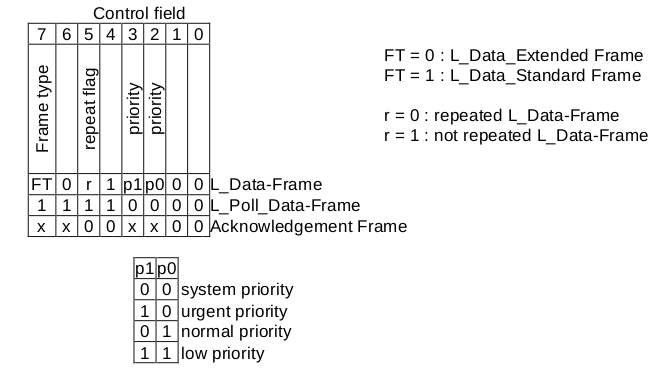
\includegraphics[width=0.5\textwidth]{figures/controlfield.png}
    \caption{Control Field}
    \label{fig:ctrlfield}
\end{figure}

Three frame formats are defined: L\_Data frames are used for sending a data payload to an individual address, a group address or for broadcasting data to
the bus. L\_Poll\_Data frames are used to request data from an individual knx device or a group of devices. Acknowledgement frames are used to provide a reliable
transport mechanism, i.e. to acknowledge the reception of a frame by a knx device. 

For L\_Data\_Frame, 2 different formats are defined: standard frames \ref{fig:stdframe} and extended frames \ref{fig:extframe}. While standard frames can bear up to
15 bytes of application data, extended frames allow the transmission of up to 254 bytes of data.

\subsubsection{Standard L\_Data\_Frame}

Every standard frame starts with the control field, determining the frame type. 
After that, sender address and destination address, each 2 byte, follow.
The next byte contains 1 address type bit, 3 bits which belong to the \gls{lsdu} of the next higher layer
and 4 bits of length information, resulting in an maximum payload of 15 bytes(by design, it is also allowed to set this length
field to 0, i.e. to send an empty data frame). After the corresponding number of payload bytes, a check byte completes the frame. This check
frame is defined as an odd parity over all preceding bytes, which represents a logical NOT XOR function. 

\begin{figure}
    \centering
    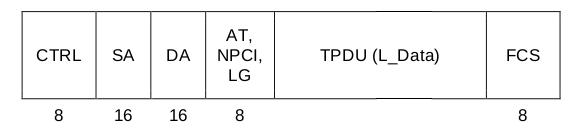
\includegraphics[width=0.5\textwidth]{figures/standardframe.png}
    \caption{Standard Frame}
    \label{fig:stdframe}
\end{figure}

\begin{figure}
    \centering
    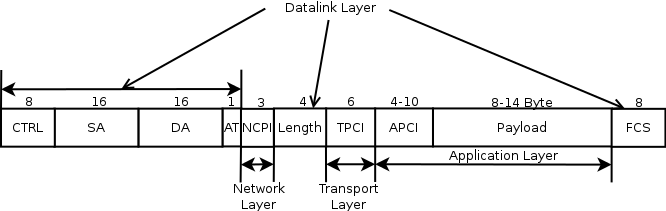
\includegraphics[width=0.5\textwidth]{figures/standardFrame.png}
    \caption{Standard Frame, in detail}
    \label{fig:stdFrameDetail}
\end{figure}


\subsubsection{Extended L\_Data\_Frame}

The extended frame starts with a control field, as a standard frame. After that, a special \gls{ctrle} follows, as shown in figure \ref{fig:ctrle}.
Source- and destination addresses, each 2 bytes, follow. To allow the bigger payload, the next byte is used as length field, with the value 0xFF reserved
as escape code. After that, the payload and the check byte, as defined above, follow.


\begin{figure}
    \centering
    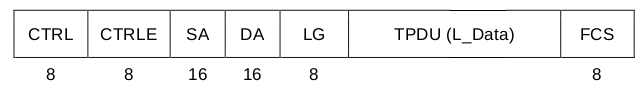
\includegraphics[width=0.5\textwidth]{figures/extendedframe.png}
    \caption{Extended Frame}
    \label{fig:extframe}
\end{figure}

\begin{figure}
    \centering
    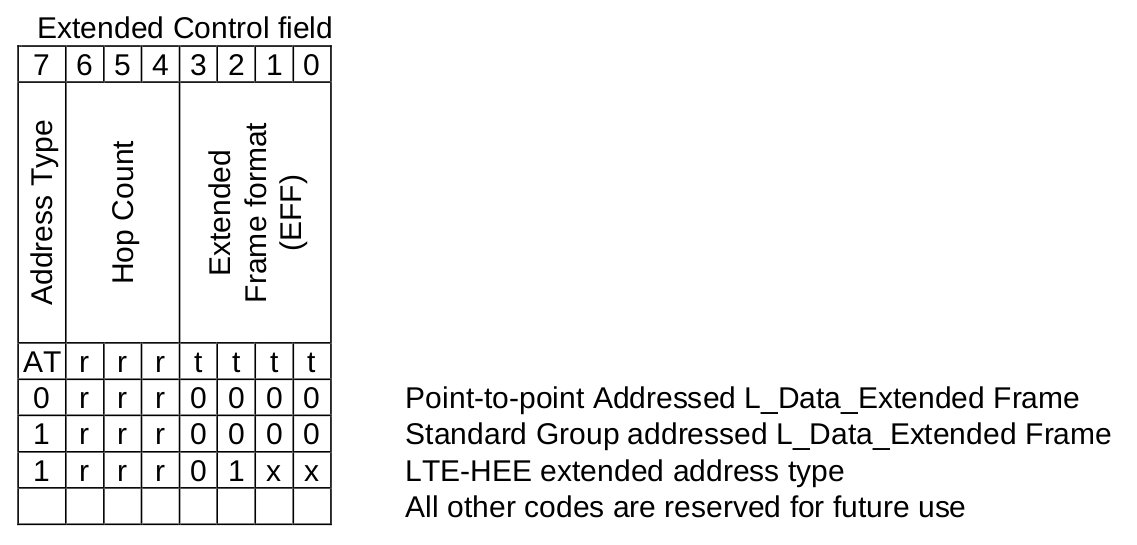
\includegraphics[width=0.5\textwidth]{figures/extendedframeCTRLE.png}
    \caption{Extended Frame CTRLE field}
    \label{fig:ctrle}
\end{figure}

\subsubsection{L\_Poll\_Data Frame}

These frames serve as data requests of the poll-data master for a maximum of 15 bytes(payload of a standard
data frame) and start with a control field, as defined, followed by the 2 byte source address
of the sender(called Poll\_Data Master). The following 2 byte destination address is 
used to address up to 15 poll slaves, all belonging to the same poll group. The number of
exptected bytes and the check octet follow.

Poll requests are answered by poll slaves by transmitting the databytes in the corresponding poll slave slot.
This is achieved by defining exact timings when each poll data slave must send the requested data. Therefor, such frames can only be used within
one physical segment \cite{knxTP1}.

\subsubsection{Acknowledge Frame}

This frames are used to acknowledge the reception of a knx data frames(FIXME: ONLY DATAFRAMES??) for group- or individual addresses and consist
of one byte, sent after a fixed timespan after reception of the frame.

\subsection{Network Layer}

The main task of the network layer is the routing and forwarding of packets, so the main parameter on this layer is the destination address of the
datagram. Additionally, \gls{knx} reserves 3 bits of every standard- and extended data frame for this task, used as
\textit{hop count}. This counter is decremented by every router and is discarded if the counter reaches the value zero. This mechanism, known from
\gls{ipv4} \cite{rfc791} \footnote{Originally, this was called \gls{ttl}}, avoids the infinite circulation of packages within an incorrectly configured network.

\subsection{Transport Layer}

This layer provides services for reliable point-to-point connections, as well as connection-less point-to-point, 
point-to-domain(multicast) and point-to-all-points(broadcast):

\begin{itemize}
 \item point-to-point, connectionless\\T\_Data\_Individual: connection-less, unreliable point-to-point

 \item point-to-point, connection orientated:
 \\T\_Connect: establish reliable connection to individual address
 \\ 
 T\_Data\_Connected: send data over established connection
 \\ 
 T\_Disconnect: terminate connection to individual address 
 \\
 This service uses a timer to detect timeouts, and allows up to 3 retransmissions. Prior to sending data, a T\_Connect request has to be sent. If the
 remote device cannot handle a new connection, a T\_Disconnect request is returned to the sender. Otherwise, no confirmation or acknowledgment is sent
 to the remote device.
 
 \item point-to-multipoint, connectionless
 \\
 T\_Data\_Group: unreliable multicast to group address

 \item point-to-all-points, connectionless
 \\
 T\_Data\_Broadcast: unreliable broadcast to all devices of a domain

 \item point-to-all-points, connectionless
 \\
 T\_Data\_SystemBroadcast: unreliable broadcast to all devices of a domain FIXME: unterschied Broadcast-SystemBroadcast
\end{itemize}

\begin{figure}
    \centering
    \includegraphics[width=0.8\textwidth]{figures/"transport flags".png}
    \caption{Flags used at the Transport Layer}
    \label{fig:tFlags}
\end{figure}
%FIXME: quellenangabe bild, KNX standard

\subsection{Session Layer}

This layer is left empty in KNX and just forwards data transparently from the lower level to the upper level, and vice versa.

\subsection{Presentation Layer}

This layer is left empty in KNX and just forwards data transparently from the lower level to the upper level, and vice versa.

\subsection{Application Layer}

\section{KNX addressing}

Two different kinds of addresses, see figure \ref{fig:knxAddr} are used: individual addresses which must be unique within the network, and group
addresses. Every \gls{knx} device
beside bridges must possess one individual address and can also be member of an arbitrary large number of group addresses.

\begin{figure}
 \centering
 \subfloat[]{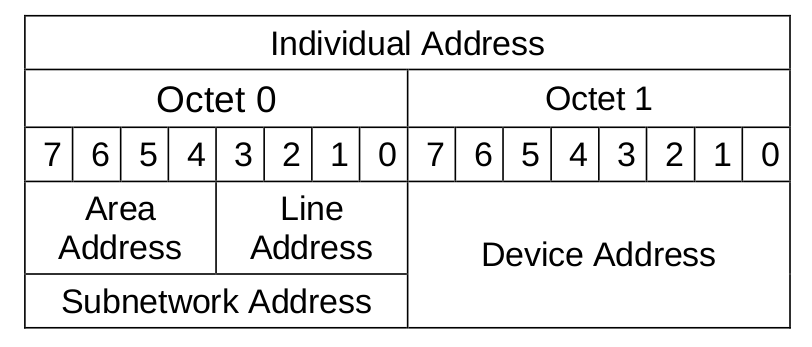
\includegraphics[width=2in]{figures/ia.png}}          
 \subfloat[]{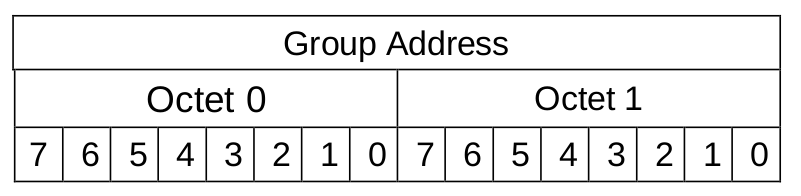
\includegraphics[width=2in]{figures/ga.png}}      
 \caption{KNX individual(a) and group(b) addresses} 
\label{fig:knxAddr}
%% \subfloat[b]{0.3\textwidth}            
\end{figure}